\documentclass[10pt]{article}
\usepackage{kotex}
\usepackage{amssymb}
\usepackage{amsmath}
\usepackage{graphicx}
\usepackage{subfigure}
\usepackage{booktabs}
\usepackage{multirow}
\usepackage{titlesec}
\usepackage[hidelinks]{hyperref}

\titleformat{\section}
  {\centering\normalfont\large\sffamily\bfseries}
  {\thesection.}
  {1em}
  {}
\titleformat{\subsection}
  {\normalfont\normalsize\sffamily\bfseries}
  {\thesubsection.}
  {1em}
  {\itshape}

\renewcommand{\thesection}{\Roman{section}}
\def\thesubsection{\arabic{subsection}}

\usepackage{setspace}
\setstretch{1.31}

\textwidth 17.6cm
\textheight 24.2cm
\addtolength{\oddsidemargin}{-25mm}
\addtolength{\topmargin}{-21mm}
\setcounter{page}{0}

\begin{document}

\begin{center}
{\LARGE \bf 잡음 비디오의 저비트레이트 H.264 인코딩을 위한 3차원 DT-CWT 전처리의 조건부 성능 분석}\\[12pt]
민찬, 지도교사\\
서울과학고등학교\\[12pt]
{\LARGE \bf Conditional Performance Analysis of 3D DT-CWT Preprocessing for Low-Bitrate H.264 Encoding of Noisy Video}\\[12pt]
Minchan, Advisor\\
Seoul Science High School\\[12pt]

{\large \bf 국문 초록}
\noindent\rule{\textwidth}{0.4pt}
\begin{flushleft}
본 연구는 잡음이 포함된 비디오를 저비트레이트 H.264/x264로 인코딩하기 전에 3차원 dual-tree complex wavelet transform(3D DT-CWT) 전처리를 적용했을 때의 조건부 성능을 분석하였다. 기존의 전처리 연구가 잡음 제거 자체의 성능을 강조하는 경우가 많았던 것과 달리, 본 연구는 입력 영상이 깨끗한 경우와 잡음이 있는 경우를 분리하고, 인코딩 전후의 성능 변화를 함께 비교하였다. 실험에는 CIF 해상도의 \textit{akiyo}, \textit{foreman} 영상을 사용하였고, 휘도 채널에 가우시안 잡음 $\sigma=0,5,10,15$를 추가한 뒤 100--500 kbps 범위에서 x264 인코딩을 수행하였다. 제안 방법은 베이스라인 x264 인코딩, x264 내부 잡음 제거, hqdn3d, 3D DWT, Gaussian blur와 비교하였다. 그 결과 깨끗한 영상에서는 제안 방법이 평균 PSNR 기준으로 \textit{akiyo}에서 -0.24 dB, \textit{foreman}에서 -0.15 dB의 소폭 열화를 보였으나, 잡음 영상에서는 잡음이 커질수록 성능이 향상되어 \textit{akiyo}에서 최대 2.82 dB, \textit{foreman}에서 최대 0.92 dB의 평균 PSNR 이득을 보였다. PSNR-B와 edge PSNR에서도 전반적으로 같은 경향이 관찰되었다. 다만 인코딩 전후의 이득 차이를 비교한 결과 codec gain은 음수로 나타나, 현재 결과는 x264가 전처리 이득을 증폭한다기보다 전처리에서 얻은 이득 일부가 인코딩 이후에도 유지된다는 해석을 지지한다. 따라서 3D DT-CWT 전처리는 항상 적용할 방식이라기보다, 입력 잡음 수준을 추정하여 선택적으로 활성화할 때 가장 적절한 방법임을 확인하였다.

\textbf{주제어:} 3D DT-CWT, 비디오 전처리, H.264, 저비트레이트 인코딩, 잡음 제거
\noindent\rule{\textwidth}{0.4pt}
\end{flushleft}

{\large \bf Abstract}
\noindent\rule{\textwidth}{0.4pt}
\begin{flushleft}
This study analyzes the conditional performance of three-dimensional dual-tree complex wavelet transform (3D DT-CWT) preprocessing before low-bitrate H.264/x264 encoding of noisy video. Unlike prior preprocessing studies that mainly emphasize denoising itself, this work separates clean and noisy inputs and compares gains before and after encoding. CIF \textit{akiyo} and \textit{foreman} sequences were corrupted with Gaussian noise of $\sigma=0,5,10,15$ on the luma channel and encoded at 100--500 kbps. The proposed method was compared with direct x264 encoding, x264 noise reduction, hqdn3d, 3D DWT, and Gaussian blur. On clean inputs, the proposed method slightly degraded mean PSNR by 0.24 dB on \textit{akiyo} and 0.15 dB on \textit{foreman}. On noisy inputs, the gain increased with noise level, reaching 2.82 dB on \textit{akiyo} and 0.92 dB on \textit{foreman}. PSNR-B and edge PSNR showed the same general trend. However, the measured codec gain was negative, indicating that the present results support preservation rather than amplification of the preprocessing benefit through x264 encoding. These findings suggest that 3D DT-CWT preprocessing should be applied conditionally according to the estimated noise level of the input video.

\textbf{Keywords:} 3D DT-CWT, video preprocessing, H.264, low-bitrate encoding, denoising
\noindent\rule{\textwidth}{0.4pt}
\end{flushleft}
\end{center}

\section{\large \bf 서론(Introduction)}
저비트레이트 비디오 압축에서는 입력 영상에 포함된 고주파 잡음이 실제 시각 정보와 구분되지 않은 채 비트레이트를 소모하므로 압축 효율을 저하시킨다. 특히 잡음이 많은 영상은 동일한 목표 비트레이트에서 더 큰 양자화 손실을 겪기 쉽고, 결과적으로 주관적 품질과 객관적 품질이 모두 나빠질 수 있다. 이를 완화하기 위해 인코딩 이전에 잡음을 줄이는 전처리 방식이 널리 사용되지만, 전처리는 항상 이롭지 않다. 입력 영상이 이미 깨끗한 경우에는 세부 구조까지 함께 제거하여 오히려 화질을 악화시킬 수 있다.

본 연구의 목적은 3차원 DT-CWT 전처리가 저비트레이트 x264 인코딩에서 어떤 조건에서 유리한지 정량적으로 확인하는 것이다. 특히 ``DT-CWT 전처리는 항상 좋은가''가 아니라 ``어떤 입력 조건에서 이득이 나타나는가''를 핵심 질문으로 삼았다. 이를 위해 깨끗한 영상과 잡음 영상을 분리하여 비교하고, 인코딩 전 전처리 자체의 효과와 인코딩 후 최종 효과를 함께 분석하였다.

\section{\large \bf 이론적 배경(Theory \& Principle)}
\subsection{Dual-Tree Complex Wavelet Transform}
DT-CWT는 두 개의 실수 웨이블릿 트리를 사용하여 복소 계수를 구성하는 변환으로, 일반적인 실수 DWT보다 시프트 불변성과 방향 선택성이 우수하다 \cite{kingsbury1999,selesnick2005}. 이러한 특성은 영상의 경계와 방향성 구조를 보존하면서 잡음을 줄이는 데 유리하다. 본 연구에서는 공간 2차원과 시간 1차원을 함께 다루는 3차원 DT-CWT를 사용하여 프레임 간 상관성까지 고려하였다.

\subsection{BayesShrink 기반 임계값 처리}
고주파 계수 $Y_h$에 대해 잡음 분산 $\sigma_n^2$와 신호 분산 $\sigma_x^2$를 추정한 뒤, 각 서브밴드에서
\begin{equation}
T = \frac{\sigma_n^2}{\sigma_x}\alpha_l
\end{equation}
의 임계값을 사용하여 soft-thresholding을 수행하였다. 여기서 $\alpha_l$은 분해 레벨에 따른 계수이다. 본 연구의 기본 실험에서는 적응형 임계값 모드를 사용하였다.

\subsection{Rate--Distortion 분석과 BD-Rate}
동일 화질에서 필요한 비트레이트 차이를 비교하기 위해 Bjontegaard Delta Rate(BD-Rate)를 사용하였다 \cite{bjontegaard2001}. BD-Rate가 음수이면 제안 방법이 동일 품질에서 더 적은 비트레이트를 필요로 함을 의미한다. 다만 RD 곡선의 화질 구간이 충분히 겹치지 않는 경우 BD-Rate가 정의되지 않을 수 있으므로, 본 연구에서는 평균 $\Delta$PSNR과 저비트레이트 구간 평균도 함께 해석하였다.

\section{\large \bf 연구 방법(Methods)}
\subsection{실험 파이프라인}
입력 Y4M 영상은 Y/U/V 채널로 분리되며, 제안 방법에서는 휘도 채널 Y에만 3D DT-CWT 전처리를 적용하였다. 이후 원본 U/V 채널과 결합하여 x264로 인코딩하였다. 시간축 경계 아티팩트를 줄이기 위해 overlap-save 방식의 청크 처리를 사용하였다. 구현은 CUDA가 가능한 환경에서는 GPU 경로를 사용하고, 그렇지 않으면 CPU 경로로 자동 전환된다.

\subsection{실험 조건}
실험 영상은 CIF 해상도의 \textit{akiyo}, \textit{foreman} 두 종류이며, 휘도 채널에 가우시안 잡음 $\sigma=0,5,10,15$를 추가하였다. 목표 비트레이트는 100, 200, 300, 400, 500 kbps이다. 비교군은 다음과 같다.
\begin{itemize}
    \item Baseline: 전처리 없는 x264 인코딩
    \item x264 NR: x264 내부 잡음 제거 옵션
    \item hqdn3d: FFmpeg 시공간 디노이저
    \item 3D DWT: Haar 기반 3차원 DWT 전처리
    \item Gaussian: 2차원 Gaussian blur 전처리
    \item Proposed: 3D DT-CWT 전처리
\end{itemize}

\subsection{평가 지표}
주요 지표로 PSNR-Y, PSNR-B, edge PSNR(EPSNR)을 사용하였다. 이외에 SSIM, GBIM, MEPR도 함께 기록하였다. 현재 결과 파일에서는 MS-SSIM과 VMAF가 유효하게 산출되지 않았으므로, 본 논문의 결론에서는 사용하지 않았다.

\subsection{전처리 전후 비교}
전처리 자체의 효과와 인코딩 이후 효과를 구분하기 위해
\begin{equation}
\Delta_{\mathrm{pre}} = Q(\text{전처리 영상}) - Q(\text{입력 영상}),
\end{equation}
\begin{equation}
\Delta_{\mathrm{post}} = Q(\text{전처리+x264}) - Q(\text{기준+x264})
\end{equation}
를 정의하고,
\begin{equation}
\text{codec gain} = \Delta_{\mathrm{post}} - \Delta_{\mathrm{pre}}
\end{equation}
를 계산하였다. codec gain이 양수이면 코덱이 전처리 이득을 증폭한 것으로 해석할 수 있고, 음수이면 전처리 이득의 일부가 인코딩 과정에서 줄어든 것으로 해석할 수 있다.

\section{\large \bf 연구 결과 및 분석(Results and Discussion)}
\subsection{잡음 수준에 따른 PSNR 변화}
표 \ref{tab:main_psnr}은 제안 방법과 baseline의 평균 PSNR 차이를 나타낸다. 깨끗한 영상에서는 제안 방법이 소폭 열세였지만, 잡음이 증가할수록 이득이 커졌다. 특히 \textit{akiyo}는 $\sigma=15$에서 2.82 dB의 뚜렷한 향상을 보였다.

\begin{table}[hbtp]
\centering
\caption{제안 방법의 평균 PSNR 이득(dB)}
\label{tab:main_psnr}
\begin{tabular}{lrrrr}
\toprule
영상 & $\sigma=0$ & $\sigma=5$ & $\sigma=10$ & $\sigma=15$ \\
\midrule
\textit{akiyo} & -0.24 & 1.34 & 2.05 & 2.82 \\
\textit{foreman} & -0.15 & 0.02 & 0.45 & 0.92 \\
\bottomrule
\end{tabular}
\end{table}

\begin{figure}[hbtp]
\centering
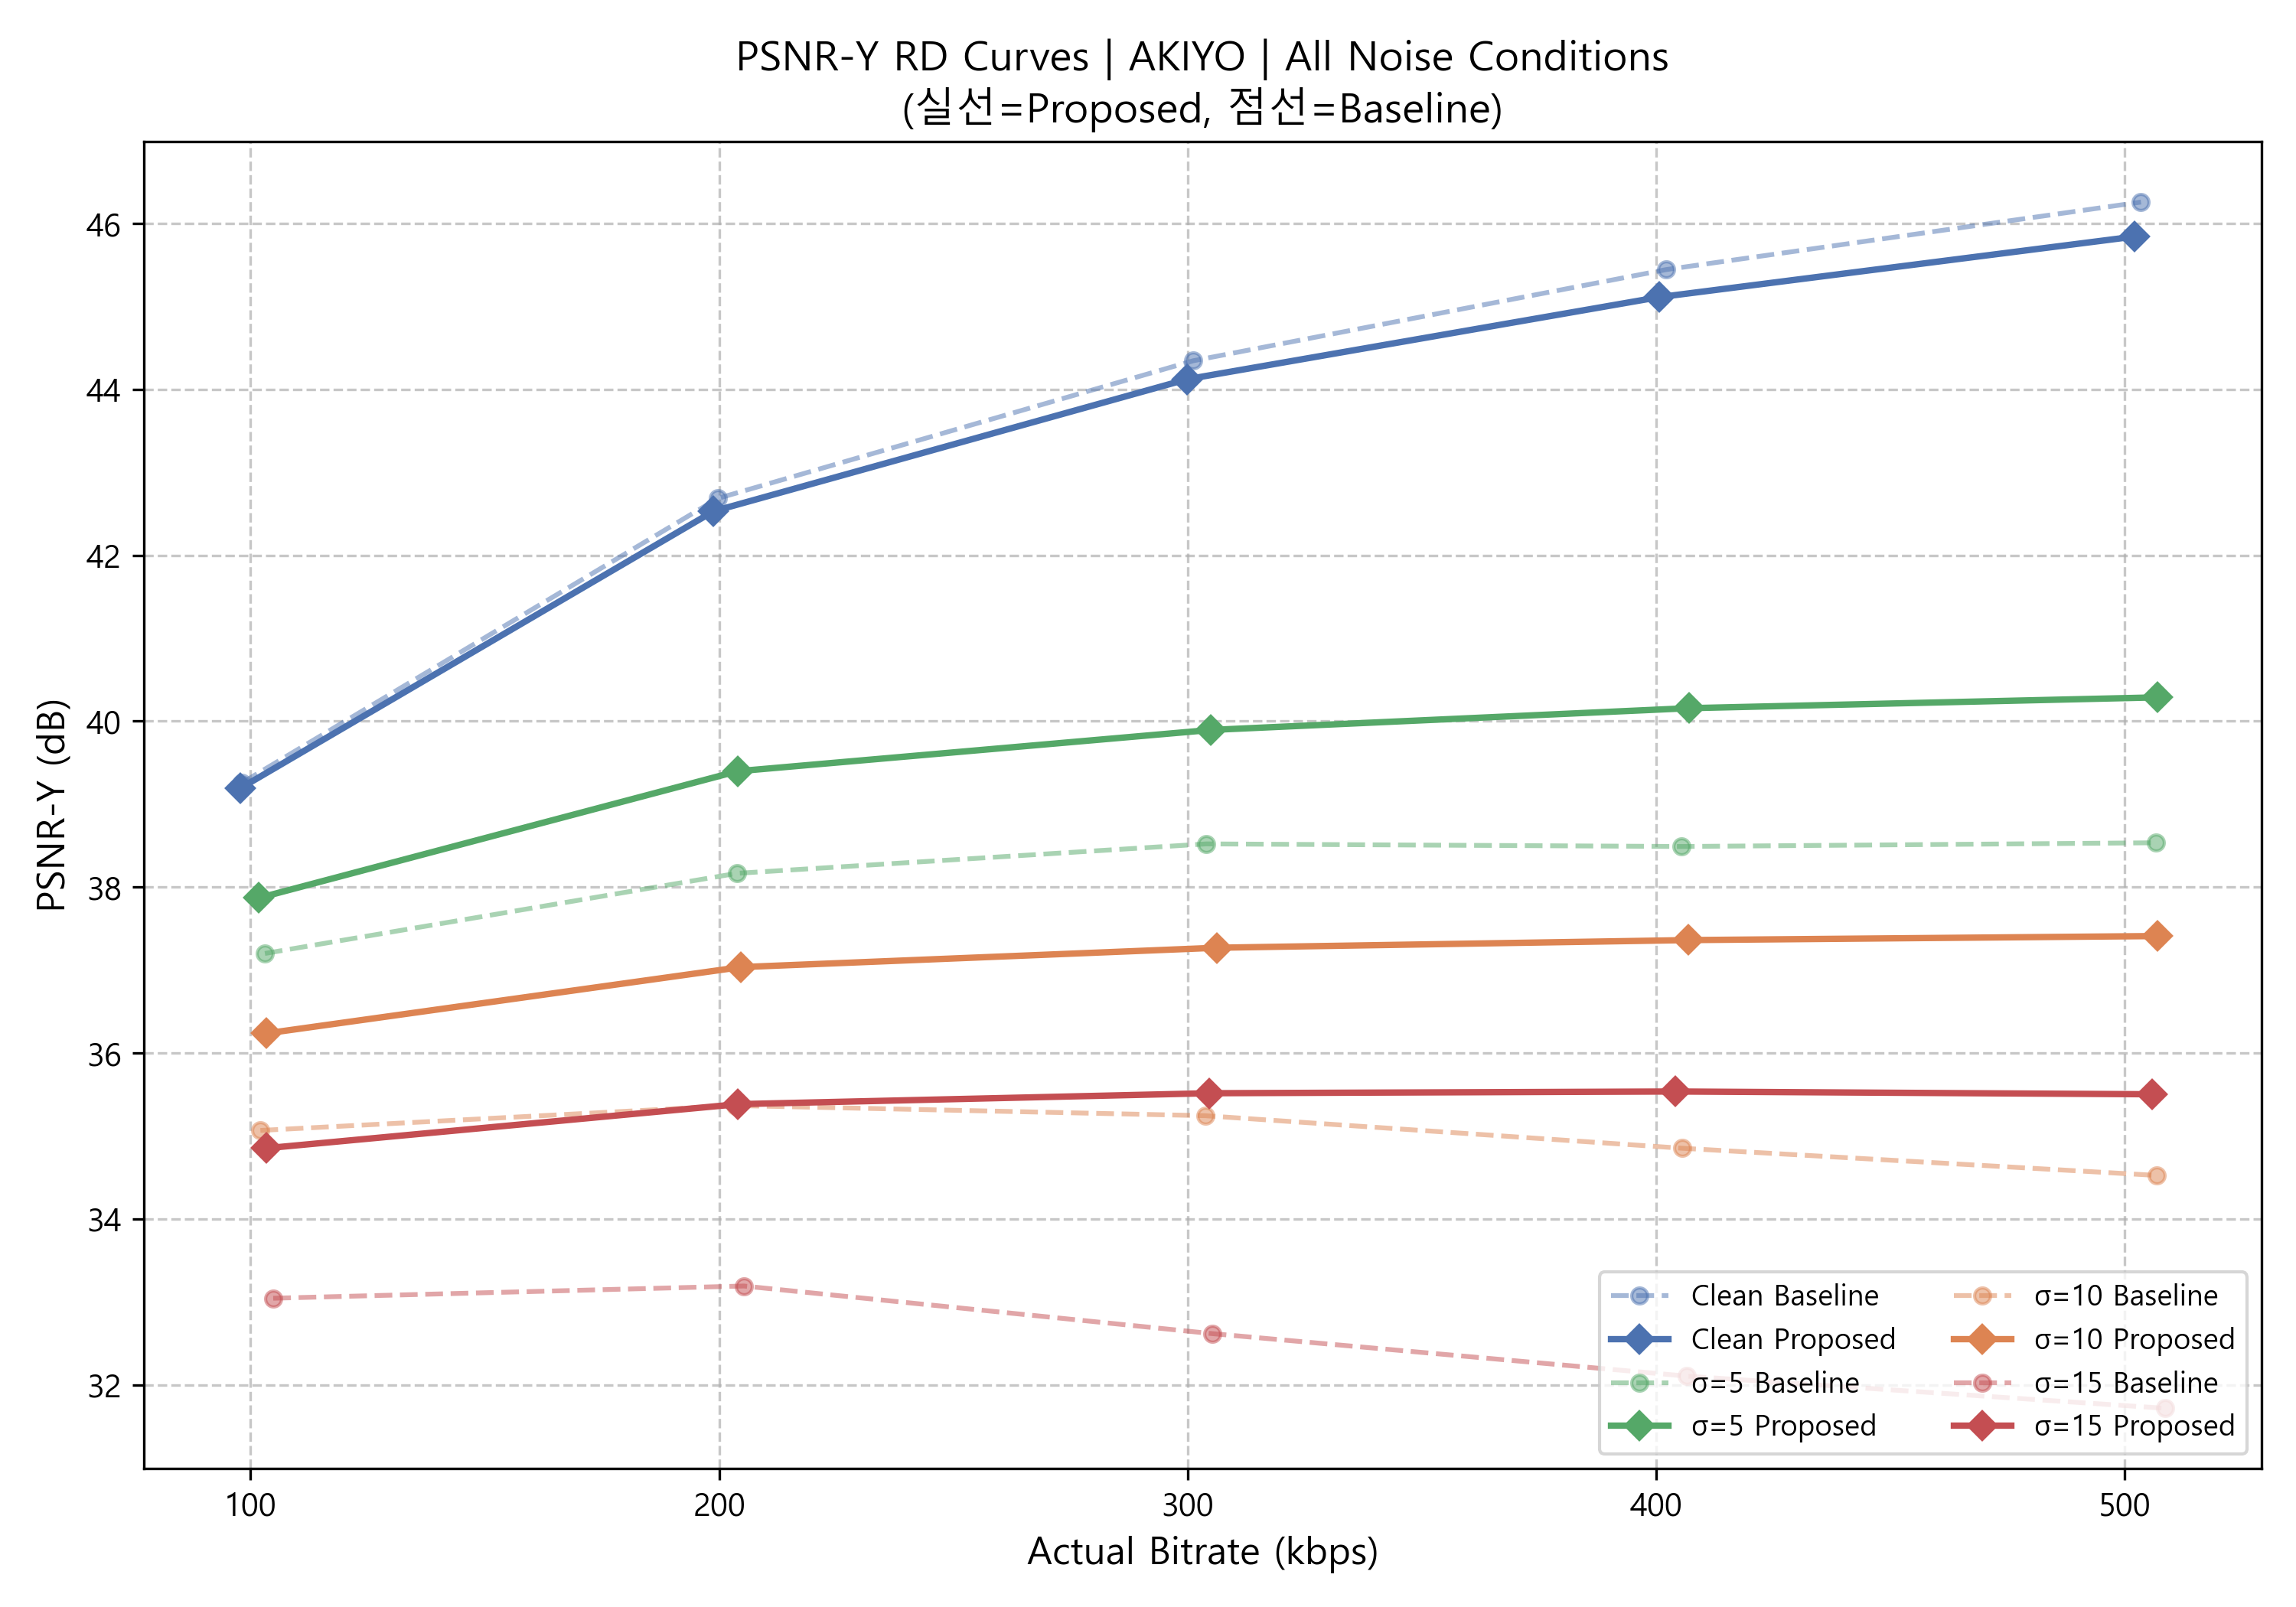
\includegraphics[width=0.78\textwidth]{../outputs/noise_experiment/rd_overlay_psnr_akiyo.png}
\caption{\textit{akiyo} 영상에서 잡음 조건별 PSNR RD 곡선}
\label{fig:akiyo_overlay}
\end{figure}

\begin{figure}[hbtp]
\centering
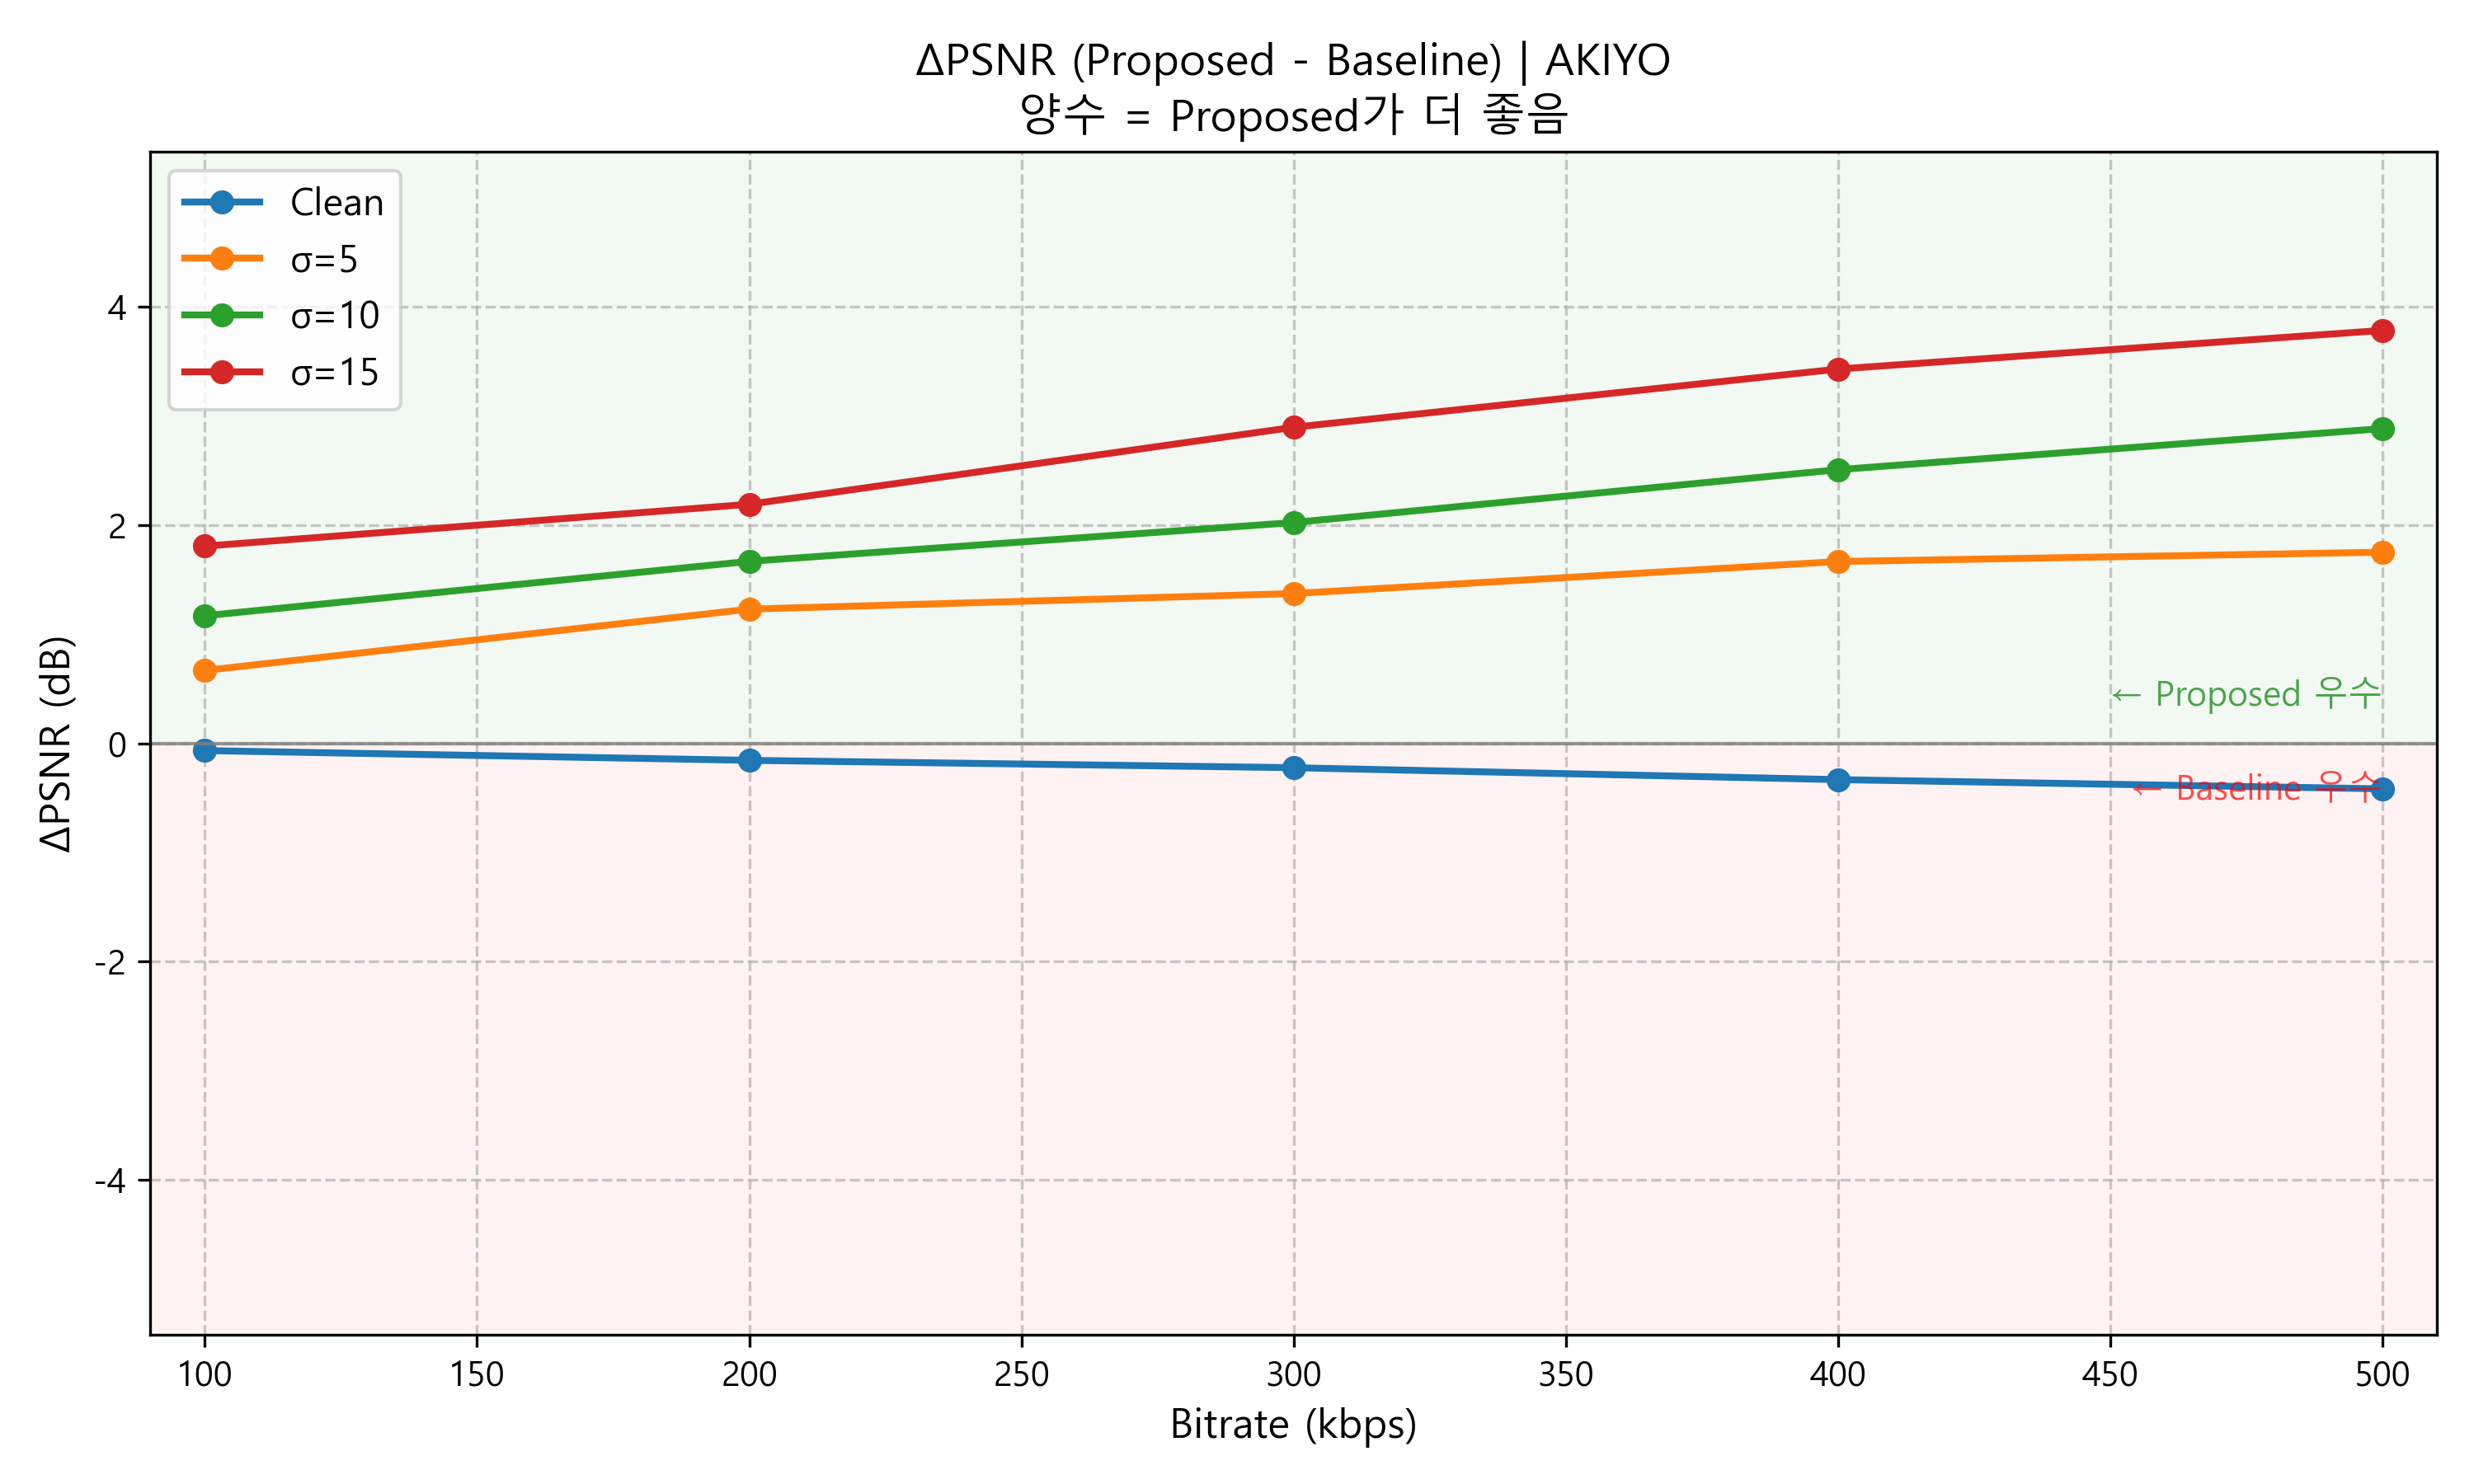
\includegraphics[width=0.72\textwidth]{../outputs/noise_experiment/delta_psnr_akiyo.png}
\caption{\textit{akiyo} 영상에서 bitrate별 $\Delta$PSNR 변화}
\label{fig:delta_akiyo}
\end{figure}

\subsection{보조 지표 분석}
표 \ref{tab:aux_metrics}는 PSNR-B와 EPSNR의 평균 이득을 보여준다. clean 조건에서는 두 지표 모두 감소하였고, noisy 조건에서는 대체로 증가하였다. 다만 \textit{foreman}의 $\sigma=5$에서는 PSNR 이득이 거의 0에 가깝고 보조 지표는 아직 음수여서, 이 조건은 제안 방법이 확실히 우세한 구간이라기보다 전환 경계에 가깝다고 볼 수 있다.

\begin{table}[hbtp]
\centering
\caption{제안 방법의 보조 지표 평균 이득(dB)}
\label{tab:aux_metrics}
\begin{tabular}{llrrr}
\toprule
영상 & 지표 & $\sigma=0$ & $\sigma=10$ & $\sigma=15$ \\
\midrule
\multirow{2}{*}{\textit{akiyo}}
& PSNR-B & -0.11 & 2.44 & 3.67 \\
& EPSNR & -0.11 & 1.22 & 1.39 \\
\midrule
\multirow{2}{*}{\textit{foreman}}
& PSNR-B & -0.08 & 0.61 & 1.75 \\
& EPSNR & -0.11 & 0.07 & 0.26 \\
\bottomrule
\end{tabular}
\end{table}

\subsection{BD-Rate 및 전처리 전후 비교}
그림 \ref{fig:bdrate}는 조건별 BD-Rate를 나타낸다. clean 조건에서는 양수, noisy 조건에서는 음수로 나타나 본 연구의 핵심 가설과 일치한다. 다만 \textit{akiyo}의 고잡음 조건 일부에서는 RD 곡선의 공통 화질 구간이 충분하지 않아 BD-Rate가 정의되지 않았고, 이 경우 평균 PSNR 이득과 저비트레이트 구간 평균을 중심으로 해석하는 것이 더 적절하다.

\begin{figure}[hbtp]
\centering
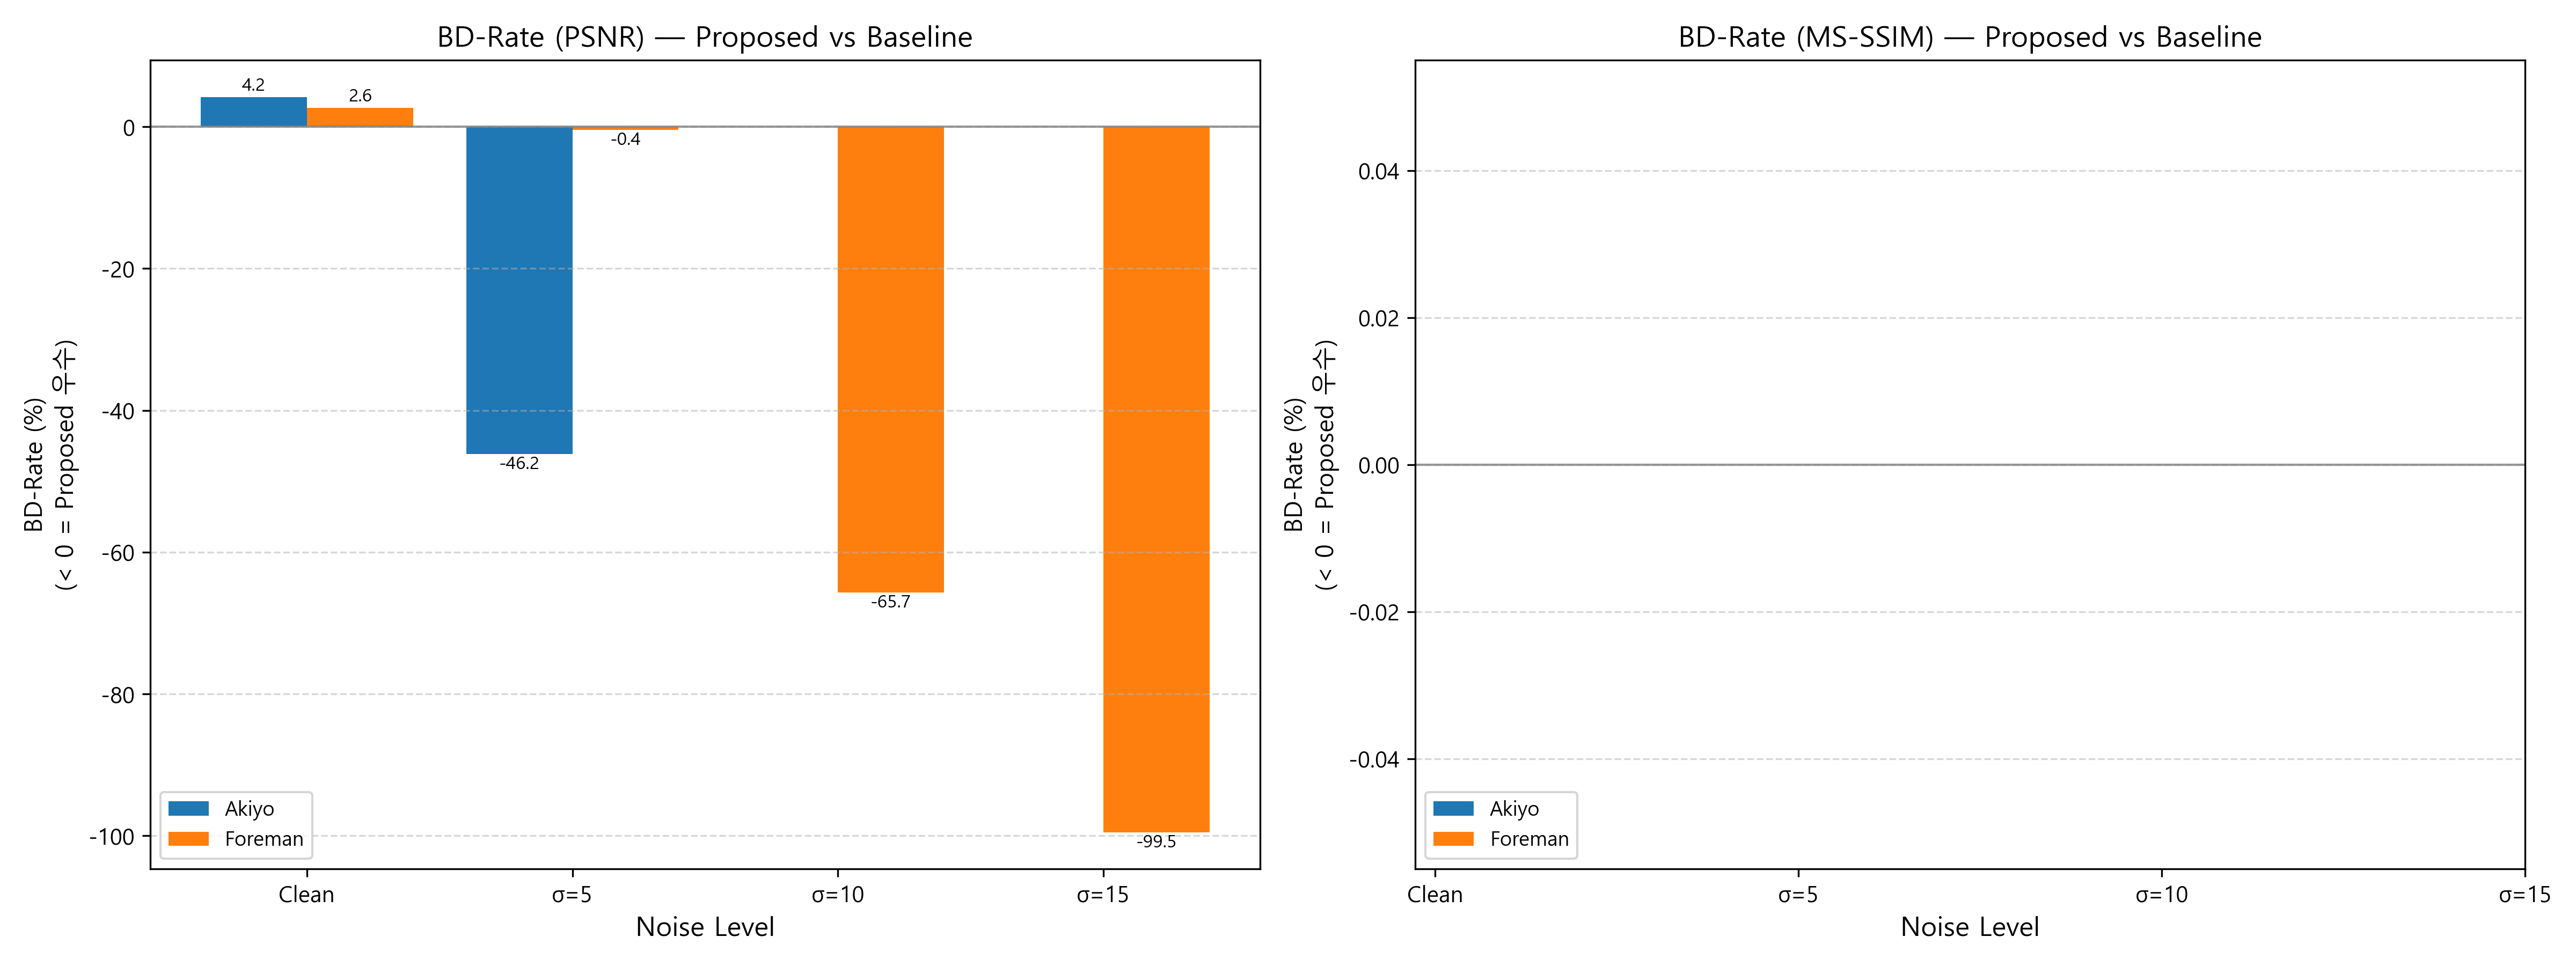
\includegraphics[width=0.78\textwidth]{../outputs/noise_experiment/cross_condition_bd_rate.png}
\caption{조건별 BD-Rate 비교}
\label{fig:bdrate}
\end{figure}

또한 그림 \ref{fig:codec_gain}과 같이 codec gain은 noisy 조건에서 모두 음수였다. 예를 들어 \textit{akiyo}의 codec gain은 $\sigma=5,10,15$에서 각각 -3.10 dB, -4.74 dB, -5.23 dB였으며, \textit{foreman}에서도 -1.93 dB에서 -4.58 dB 사이였다. 따라서 본 연구 결과는 ``x264가 DT-CWT 전처리 효과를 증폭한다''는 강한 해석보다는, ``전처리 자체의 이득이 인코딩 이후에도 일부 유지된다''는 해석을 지지한다.

\begin{figure}[hbtp]
\centering
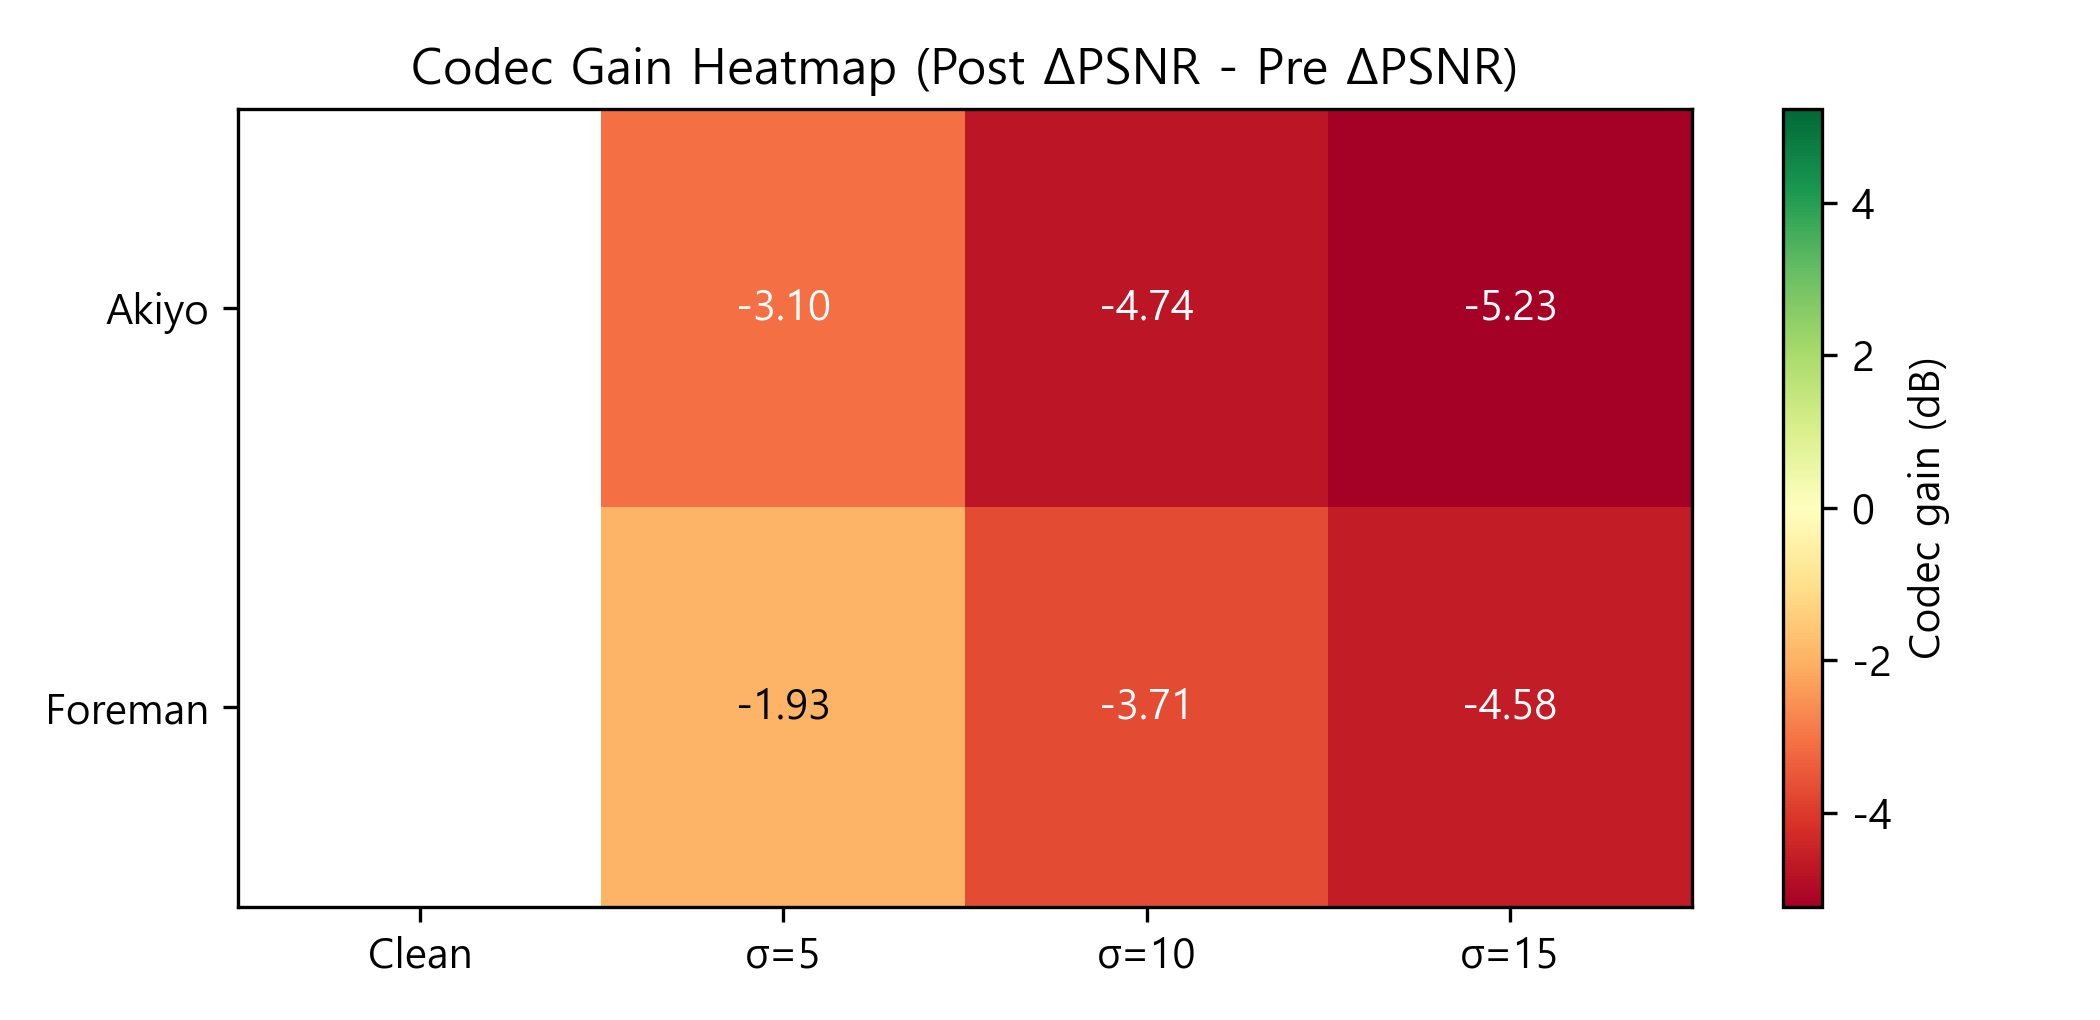
\includegraphics[width=0.68\textwidth]{../outputs/noise_experiment/codec_gain_heatmap.png}
\caption{조건별 codec gain heatmap}
\label{fig:codec_gain}
\end{figure}

\section{\large \bf 결론 및 제언(Conclusion and Proposal)}
본 연구는 3D DT-CWT 전처리가 저비트레이트 H.264 인코딩에서 입력 영상의 잡음 수준에 따라 상반된 효과를 보인다는 점을 확인하였다. 깨끗한 영상에서는 소폭의 성능 저하가 나타났지만, 잡음이 포함된 영상에서는 잡음 수준이 커질수록 평균 PSNR, PSNR-B, EPSNR이 향상되었다. 특히 저비트레이트 환경에서 \textit{akiyo} 영상은 뚜렷한 개선을 보였다.

따라서 실제 시스템에서는 DT-CWT 전처리를 항상 적용하기보다, 먼저 입력 잡음 수준을 추정한 뒤 일정 기준 이상에서만 활성화하는 조건부 전략이 더 적절하다. 향후 연구에서는 더 다양한 영상 시퀀스를 포함하고, 유효한 MS-SSIM 및 VMAF 측정을 확보하며, 장면 변화와 움직임 정보를 함께 이용하는 전처리 활성화 정책을 설계할 필요가 있다.

\section*{\large \bf 보충 자료(Supplemental Information)}
\appendix
\renewcommand{\theequation}{A.\arabic{equation}}
\setcounter{equation}{0}
\subsection{\large \bf 주요 결과 파일}
본 연구의 원자료는 \texttt{outputs/noise\_experiment/raw\_data\_*} 파일에 저장되었고, 요약표는 \texttt{summary\_bd\_rates.csv}, \texttt{summary\_reliable\_metrics.csv}에 저장되었다. 그래프는 동일 디렉터리의 PNG 파일로 생성하였다.

\begingroup
\titleformat*{\section}{\centering\normalfont\large\sffamily\bfseries}
\begin{thebibliography}{100}
\bibitem{kingsbury1999}
N.~G. Kingsbury,
``The dual-tree complex wavelet transform: a new technique for shift invariance and directional filters,''
\emph{Proc. IEEE Digital Signal Processing Workshop}, 1999.

\bibitem{selesnick2005}
I.~W. Selesnick, R.~G. Baraniuk, and N.~C. Kingsbury,
``The dual-tree complex wavelet transform,''
\emph{IEEE Signal Processing Magazine}, vol.~22, no.~6, pp.~123--151, 2005.

\bibitem{bjontegaard2001}
G.~Bjontegaard,
``Calculation of average PSNR differences between RD-curves,''
ITU-T VCEG-M33, 2001.
\end{thebibliography}
\endgroup

\end{document}
